% !TeX spellcheck = de_CH
%%%%%%%%%%%%%%%%%%%%%%%%%%%%%%%%%%%%%%%%%%%%%%%%%%%%%%%%%%%%%%%%%
%  _____   ____  _____                                          %
% |_   _| /  __||  __ \    Institute of Computitional Physics   %
%   | |  |  /   | |__) |   Zuercher Hochschule Winterthur       %
%   | |  | (    |  ___/    (University of Applied Sciences)     %
%  _| |_ |  \__ | |        8401 Winterthur, Switzerland         %
% |_____| \____||_|                                             %
%%%%%%%%%%%%%%%%%%%%%%%%%%%%%%%%%%%%%%%%%%%%%%%%%%%%%%%%%%%%%%%%%
%
% Project     : BA Welti Keller
% Title       : 
% File        : bedienung.tex Rev. 00
% Date        : 15.09.2014
% Author      : Tobias Welti
%
%%%%%%%%%%%%%%%%%%%%%%%%%%%%%%%%%%%%%%%%%%%%%%%%%%%%%%%%%%%%%%%%%

\chapter{Bedienungsanleitung}\label{chap.bedienung}
\todo{Bedienungsanleitung}

\section{Produktbeschrieb}\label{sec.manualproduct}
Die Messstation wurde entwickelt, um Geschiebemessungen in einem Bach oder Fluss zu machen. Als Vorbild hat eine Messstation mit \glspl{geophon} als \glspl{sensor} gedient, die einen Embedded-PC als Auswertungsrechner einsetzt. Der bauliche Aufwand für eine solche Messstation ist ziemlich gross, da viele Kabel verlegt und vor dem Geschiebe geschützt werden müssen. Mit dem Ziel, den Aufwand für die Konstruktion und die Verkabelung zu reduzieren, wurde eine neue Messstation entwickelt, die über ein Bussystem kommuniziert und die Messdaten gleich am Sensor auswertet. Auf diese Weise müssen nur noch die gewünschten, vorher spezifizierten Messdaten übertragen und gespeichert werden.

Mit der neuen Messstation können bis zu 20 Sensoren an einer Kontrolleinheit angeschlossen werden, die alle Messdaten aufzeichnet. Diese Anzahl kann nach eingehenden Tests wahrscheinlich noch erhöht werden. Die Obergrenze wird auch von der gewünschten Messdatenqualität abhängen, da das Bussystem eine begrenzte Übertragungskapazität hat.









\section{Aufbau der Messstation}\label{sec.manualoverview}
Die Messstation besteht aus einem \gls{logger} der über ein \gls{bussys} mit den \glspl{sensoreinh} verbunden ist. Die Stromversorgung (12~V Gleichspannung) erfolgt über zwei zusätzliche Leitungen im gleichen Kabel wie für das Bussystem verwendet wird. Das Kabel verläuft vom \gls{logger} zu \gls{sensoreinh} zu \gls{sensoreinh}.

\todo{bildchen des Aufbaus der Messstation}

Stromversorgung, Verdrahtung, Can-Bus, Terminator, R2D2, C3PO

Die \glspl{sensoreinh} sind in einem wasserdichten Gehäuse verbaut und über wasserdichte Steckverbinder (IP68) untereinander verbunden. 










\section{Datenlogger}\label{sec.manuallogger}
Das Herzstück der Anlage ist der \gls{logger}, der die Kontrolle über die Kommunikation hat, die Messdaten speichert und den Anschluss eines \gls{compi}s für die Konfiguration der Anlage ermöglicht. Im Datenlogger arbeitet ein \emph{ARM Cortex-M4} Prozessor mit 120~MHz Taktgeschwindigkeit. Dieser Prozessor steuert die Kommunikation und wandelt die Messdaten für die Speicherung in lesbare Information um.

\subsection{Anschlüsse}
Der \gls{logger} verfügt über vier Anschlüsse. 

\todo{figur über den logger}
\subsubsection{Stromversorgung}
Ein Anschluss ist für die Stromversorgung. Hier werden \ensuremath{12 V} Gleichspannung angeschlossen. Der Stromverbrauch ist abhängig von der Anzahl angeschlossener Sensoren.
\todo{Stromverbrauch logger und pro sensor nennen}

\subsubsection{Busanschluss}
Über den zweiten Anschluss wird das Kabel des \gls{bussys}s angeschlossen. Der Steckverbinder ist wasserdicht (IP68, Binder), damit kein Regen- oder Kondenswasser in den \gls{logger} eindringen kann. Die Messstation verwendet CAN-Bus für die Kommunikation, da dieser Standard ein sehr robustes Protokoll für die Sicherstellung der korrekten und fehlerfreien Übertragung hat. 

\subsubsection{Schnittstelle zum Computer}
Ein wasserdichter Steckverbinder für ein \gls{usb}-Kabel erlaubt den Anschluss eines Computers oder auch einen Smartphones. Über eine serielle Schnittstelle kann dann die Messstation konfiguriert werden. Der Anschluss eines \gls{compi}s und die Konfiguration ist in den Abschnitten \ref{ssec.manualserial} bis \ref{ssec.befehle} ab Seite \pageref{ssec.manualserial} im Detail beschrieben.

\subsubsection{Speicherkarte}
Die Speicherkarte kann über einen wasserdichten Schraubdeckel ausgewechselt werden, ohne dass das ganze Gehäuse des \gls{logger}s geöffnet werden muss. Der Umgang mit der Speicherkarte ist im Abschnitt \ref{sssec.sdformat} ab Seite \pageref{sssec.sdformat} erklärt.











\section{Sensor}\label{sec.manualsensor}
Die \gls{sensoreinh} der Anlage verfügen über einen Beschleunigungssensor und einen Mikroprozessor. Der Sensor misst über die Beschleunigung die Vibrationen, die vom Einschlag des Geschiebes verursacht werden. Der Mikroprozessor wertet die Messdaten aus und erkennt nach vorher definierten Kriterien die Ereignisse, deren Daten gesammelt werden sollen. Diese bereinigten Daten werden dann über das \gls{bussys} an den \gls{logger} übertragen.

\subsection{Beschleunigungssensor}
Der Beschleunigungssensor (\emph{Analog Devices ADXL001-70}) misst Beschleunigungen zwischen -70~g und +70~g. Ein g entspricht der Beschleunigung durch die Erdanziehungskraft, ungefähr 10~\ensuremath{m/s^2}. Sollten die Vibrationen stärkere Beschleunigungen erzeugen, kann entweder die Konstruktion der Messanlage angepasst werden um die Vibrationen schwächer zu machen, oder der Sensor ausgewechselt werden. Aus der Baureihe \emph{ADXL001} von \emph{Analog Devices} sind auch Sensoren mit Messbereichen von \ensuremath{\pm}250 g und \ensuremath{\pm}500 g erhältlich. Diese Modelle geben Messsignale im gleichen Spannungsbereich aus wie das verwendete Modell ADXL001-70 und können daher ohne Umkonfiguration oder Anpassungen an der \gls{software} verwendet werden.

\subsection{A/D-Wandler}
Die Messsignale vom Beschleunigungssensor werden von einem 12-Bit-\gls{adwandler} digitalisiert. Der \gls{adwandler} kann theoretisch mit bis zu 200000~Hz betrieben werden.


\subsection{Mikroprozessor}
Der \emph{ARM Cortex-M4} mit 120~MHz Taktfrequenz hat weit mehr Rechenleistung, als für die vorliegende Anwendung benötigt wird. Sollten komplexere Algorithmen für die Erkennung von Ereignissen, für die Filterung der Messdaten oder für die Verarbeitung der Signale benötigt werden, wäre dies dank der bereits vorhandenen Rechenleistung möglich.

\subsection{Anschlüsse}
Die \gls{sensoreinh} hat zwei Anschlüsse für das Bussystem. Mit dieser Bauweise ist es möglich, die \gls{stichleitung} zum \gls{transceiver} möglichst kurz zu halten, um die Signalqualität möglichst wenig negativ zu beeinflussen. Die Anschlüsse sind wasserdicht (IP68).














\section{Bussystem}\label{sec.manualbus}
Als Bussystem wird CAN-Bus verwendet. Mit einer Datenübertragungsrate von 1~MBit/s bis zu einer Kabelgesamtlänge von 40~m, resp 125~kBit/s bis zu 500~m eignet sich CAN-Bus für diese Messstation sehr gut. Es sind keine Kabellängen zu erwarten, die weit über 40~m hinausgehen. CAN-Bus ist des Weiteren sehr robust gegenüber Umwelteinflüssen, die die Übertragung stören könnten.

\subsection{Kabel}
Die Kabel der Messstation verfügen über 4 Leitungen, die jeweils paarweise verdrillt sind. Zusätzlich zu den Leitungen ist eine Zugentlastung zum Schutz vor mechanischer Beschädigung im Kabel enthalten. Um die zwei Aderpaare und die Zugentlastung ist ein metallisches Geflecht als Schild angebracht, das sowohl gegen mechanische Beschädigung als auch gegen elektrische Störeinflüsse schützt. Die PVC-Hülle des Kabels ist noch ein zusätzlicher mechanischer Schutz. 

Ein Aderpaar wird für die Spannungsversorgung verwendet, das zweite Aderpaar für die Kommunikation auf dem Bussystem.

\subsection{Abschlusswiderstände}
Damit die Bus-Signale an den Enden der Leitung nicht reflektiert werden und die Übertragung stören, müssen an beiden Enden des Bussystems Abschlusswiderstände eingesetzt werden.  Die Abschlusswiderstände (120 \ensuremath{\ohm}) verbinden die Anschlüsse CANH und CANL auf der Leiterplatte und werden wie in Abbildung \ref{fig.terminator} angebracht.

\begin{figure}
	\centering
		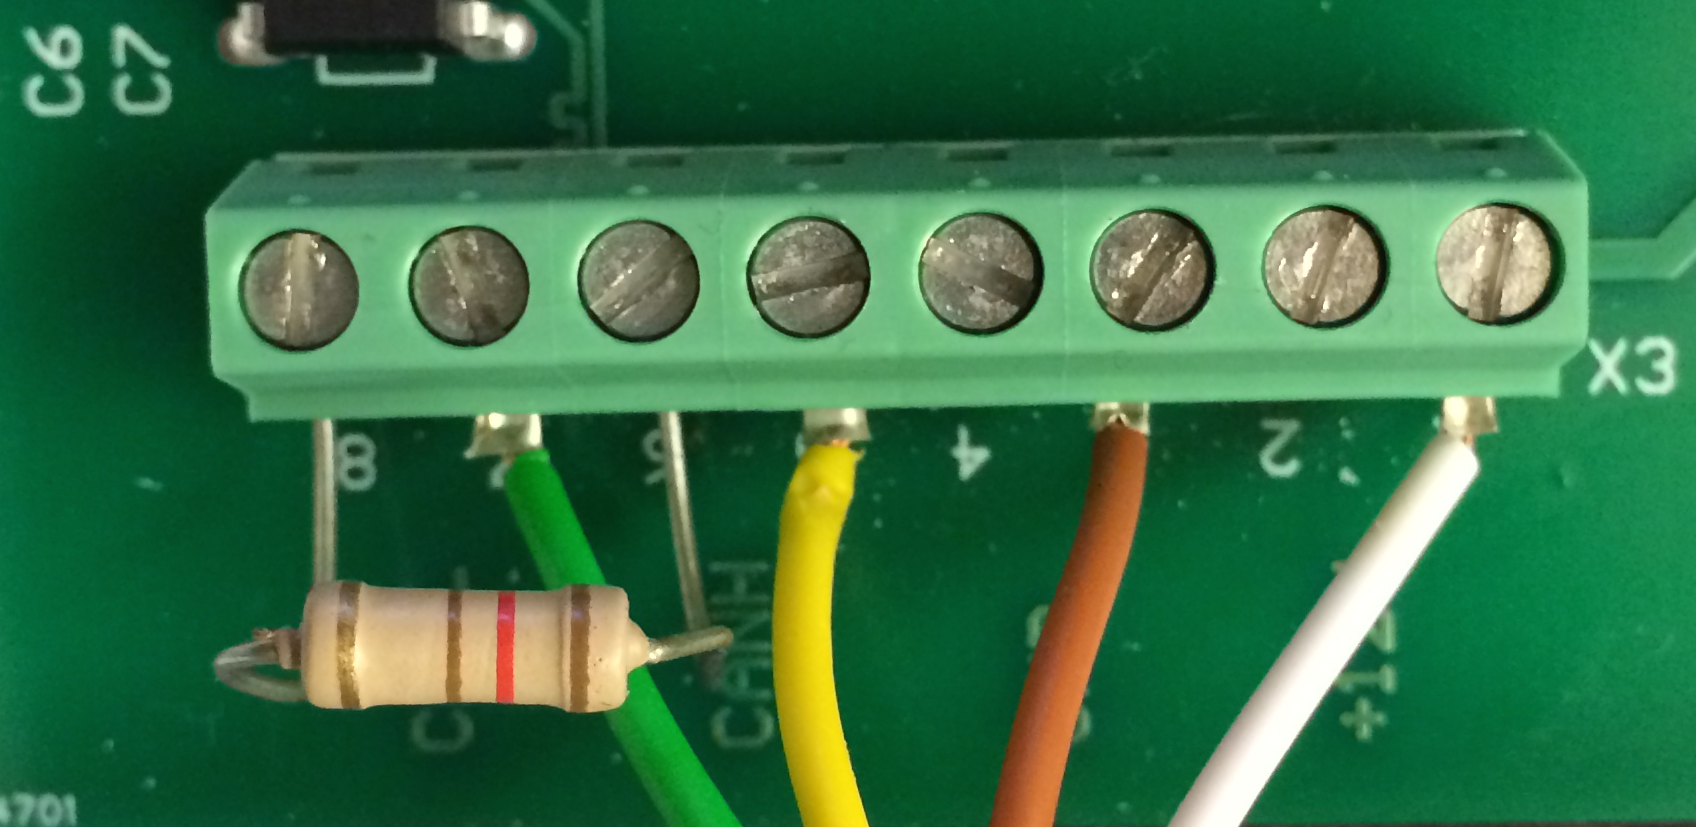
\includegraphics[width=0.8\textwidth]{images/fotos/terminator.png}
	\caption{Anbringung des \gls{terminator}s.}
	\label{fig.terminator}
\end{figure}

\subsection{Steckverbinder}
Die Steckverbinder sind fünfpolig und wasserdicht (IP68). Die Pole sind gemäss Tabelle \ref{table.stecker} bestückt, die Polnummerierung in Stecker und Buchse sind in den Abbildungen \ref{fig.polbuchse} und \ref{fig.polstecker} dargestellt.

\begin{table}
\begin{tabular}{|l|l|l|l|}
\hline \textbf{Pol Nr.}      & \textbf{Leitung} & Anschluss Schraubklemme & Aderfarbe\\ 
\hline 1 & Spannungsversorgung +12~V & +12V & weiss \\
\hline 2 & Spannungsversorgung 0~V & GND & braun \\
\hline 3 & unbenutzt &  &  \\
\hline 4 & CAN-Bus High & CANH & gelb \\
\hline 5 & CAN-Bus Low & CANL & grün \\
\hline 
\end{tabular}
\caption{Steckerbestückung des \gls{bussys}s.}
\label{table.stecker}
\end{table}  

\begin{figure}
\centering
\begin{minipage}{0.5\textwidth}
\centering
		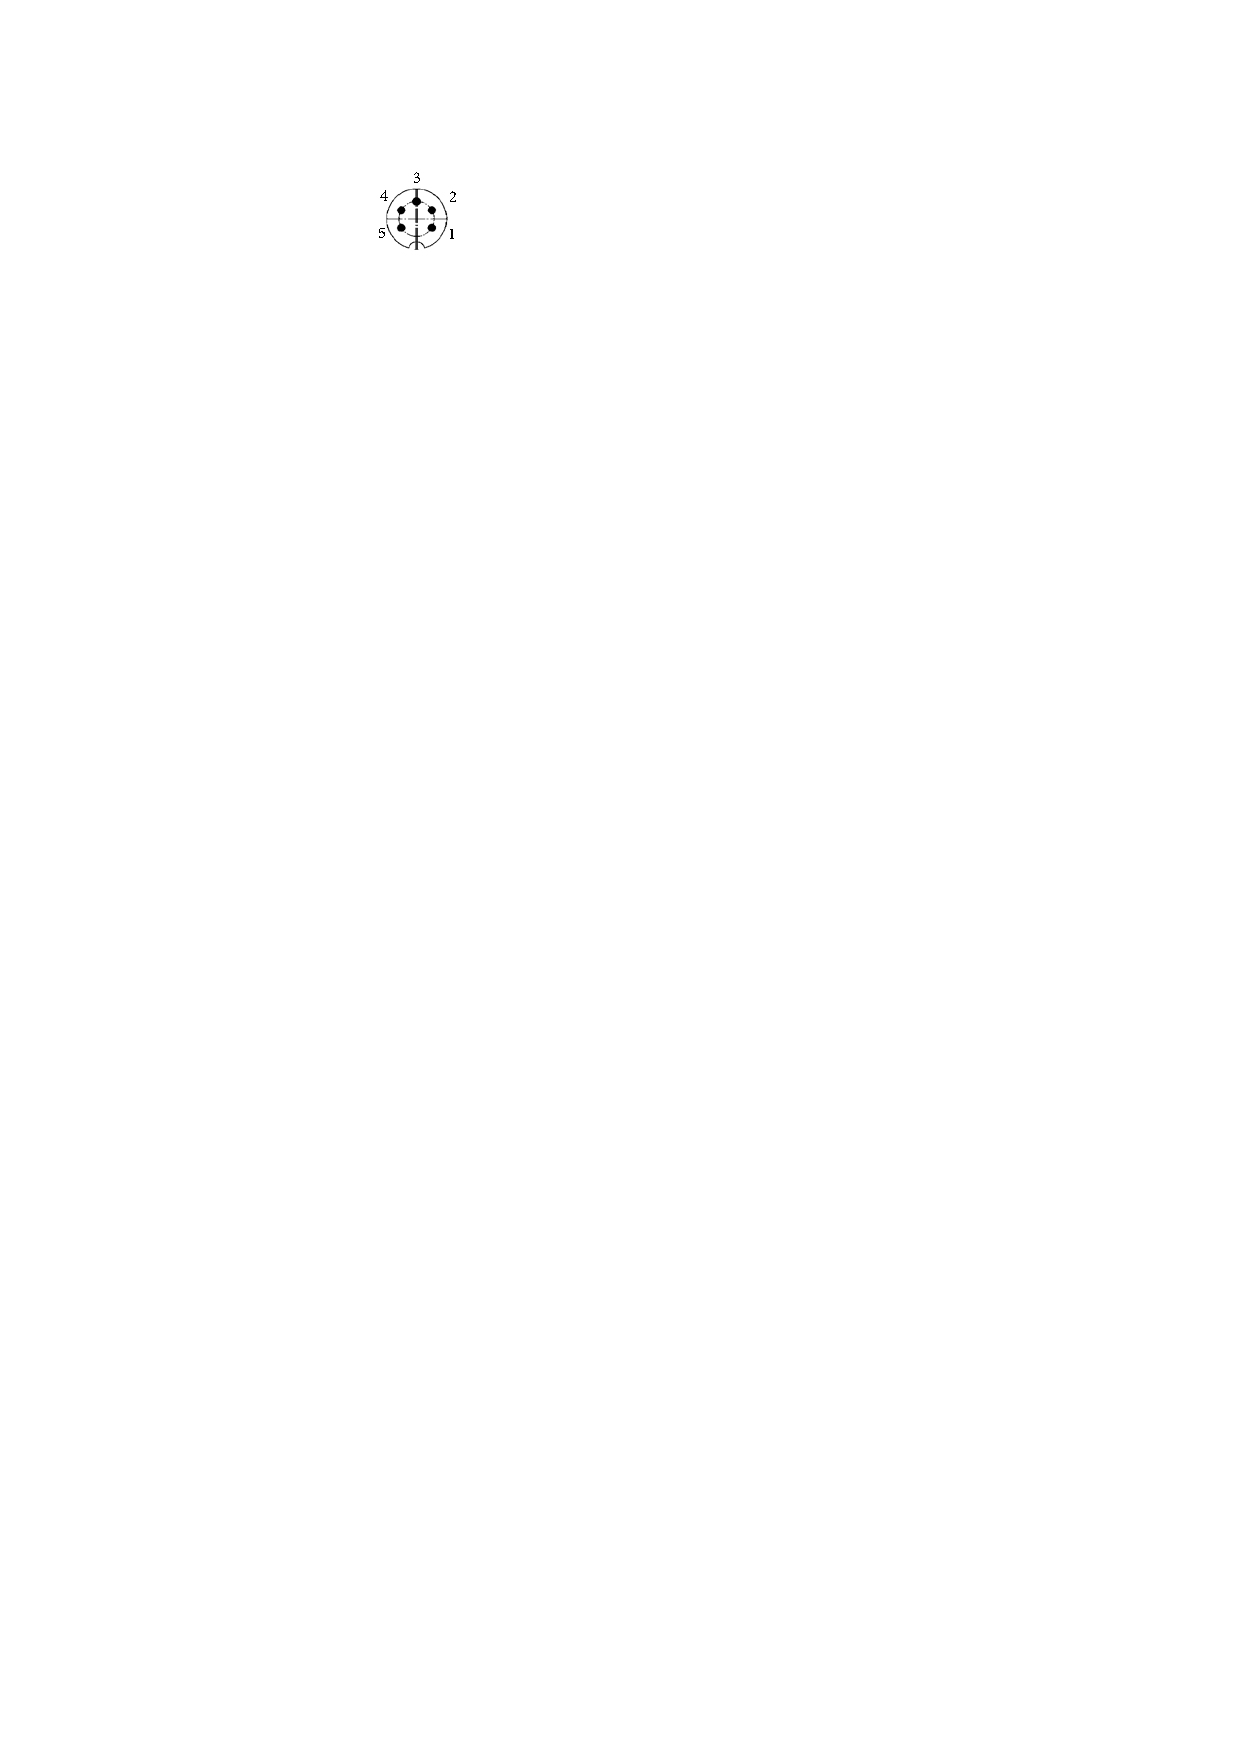
\includegraphics[width=0.8\textwidth]{images/Polbelegung_Buchse.pdf}
	\captionof{figure}{Polnummerierung in der Buchse.}
	\label{fig.polbuchse}
\end{minipage}%
\begin{minipage}{0.5\textwidth}
\centering
		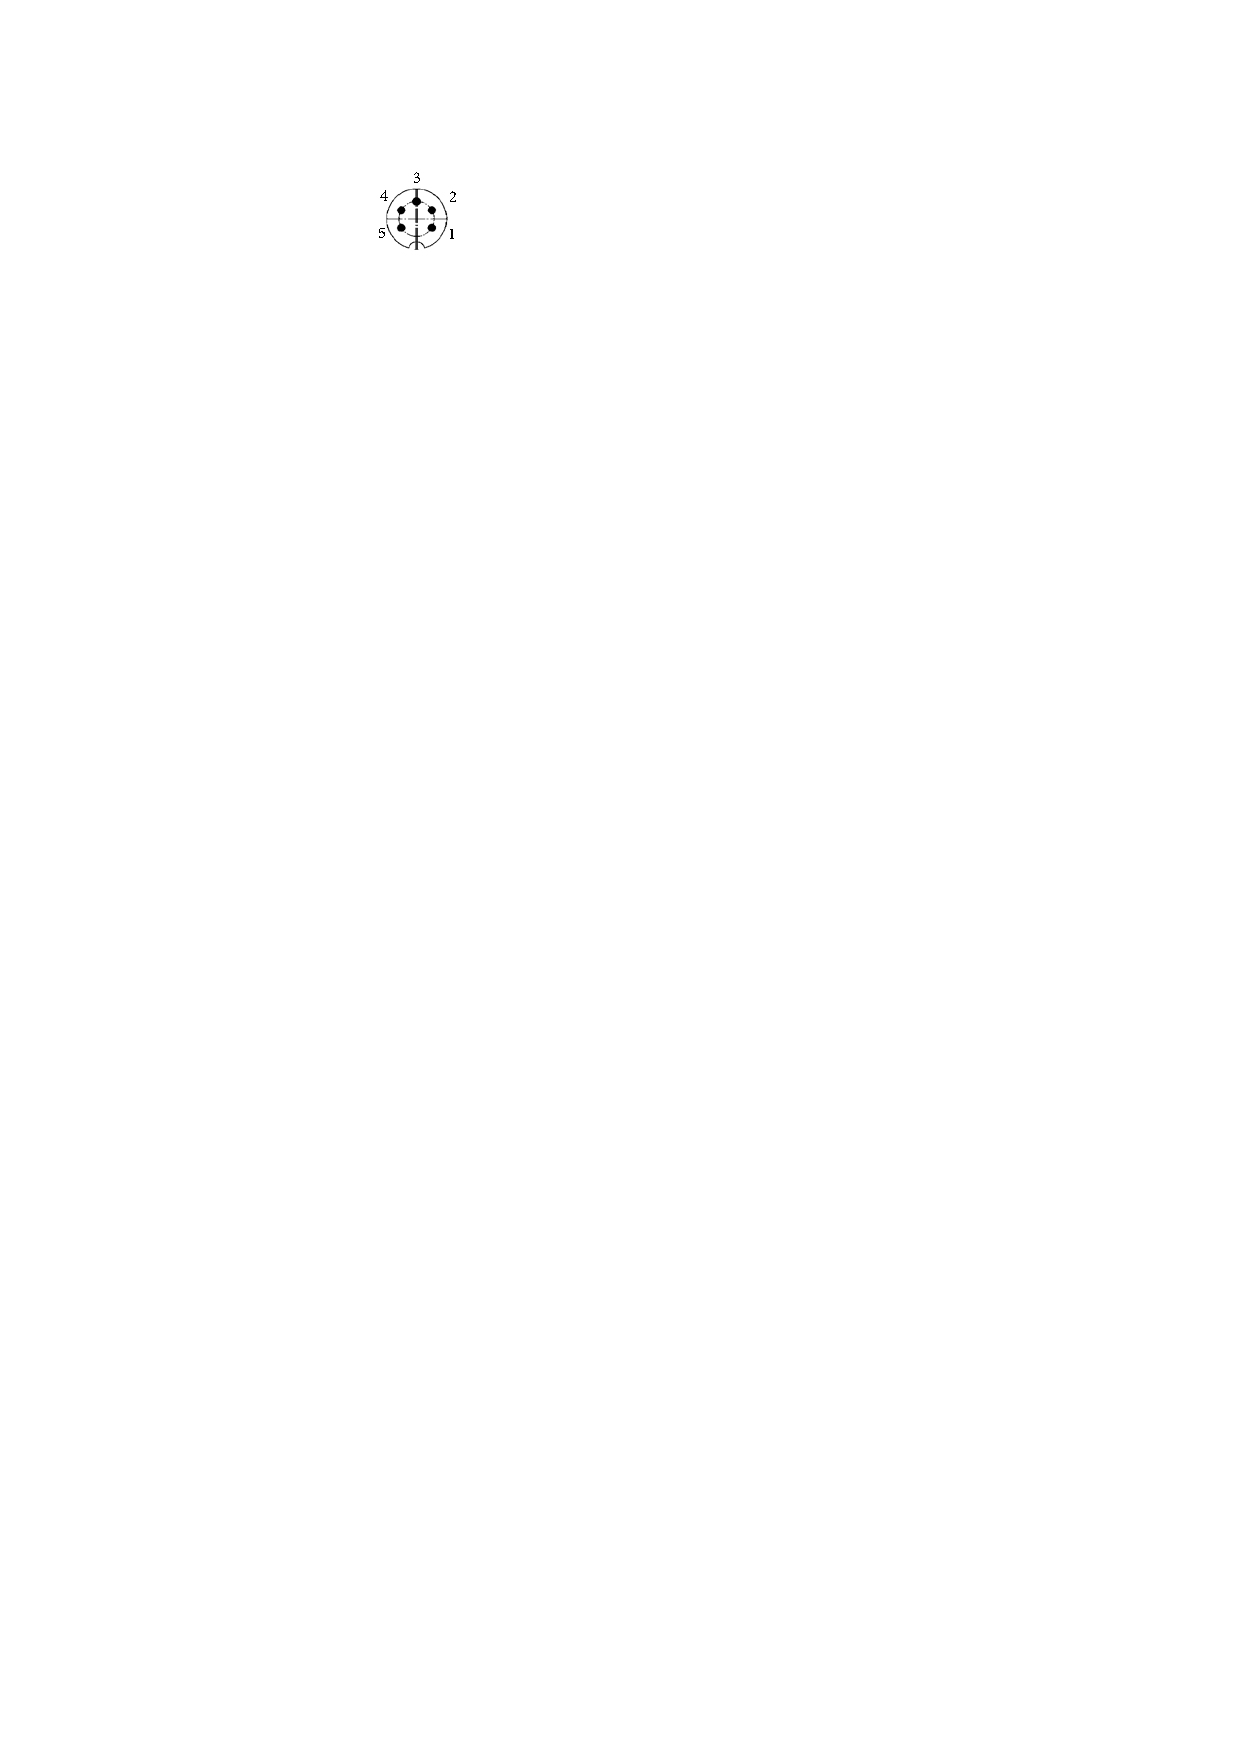
\includegraphics[width=0.8\textwidth]{images/Polbelegung_Stecker.pdf}
	\captionof{figure}{Polnummerierung im Stecker.}
	\label{fig.polstecker}
\end{minipage}
\end{figure}

Auf der Leiterplatte der \gls{sensoreinh} ist eine Schraubklemmenleiste mit 8 Anschlüssen angebracht. Hier werden die von den Buchsen kommenden Leitungen angeschlossen. Jeweils zwei benachbarte Anschlüsse sind zusammengeschaltet, damit jede Leitung einzeln fest verschraubt werden kann (Abbildung \ref{fig.kabel}). Es wird nicht empfohlen, zwei gleiche Leitungen in einer einzelnen Schraubklemme zusammen zu verschrauben.

\begin{figure}
	\centering
		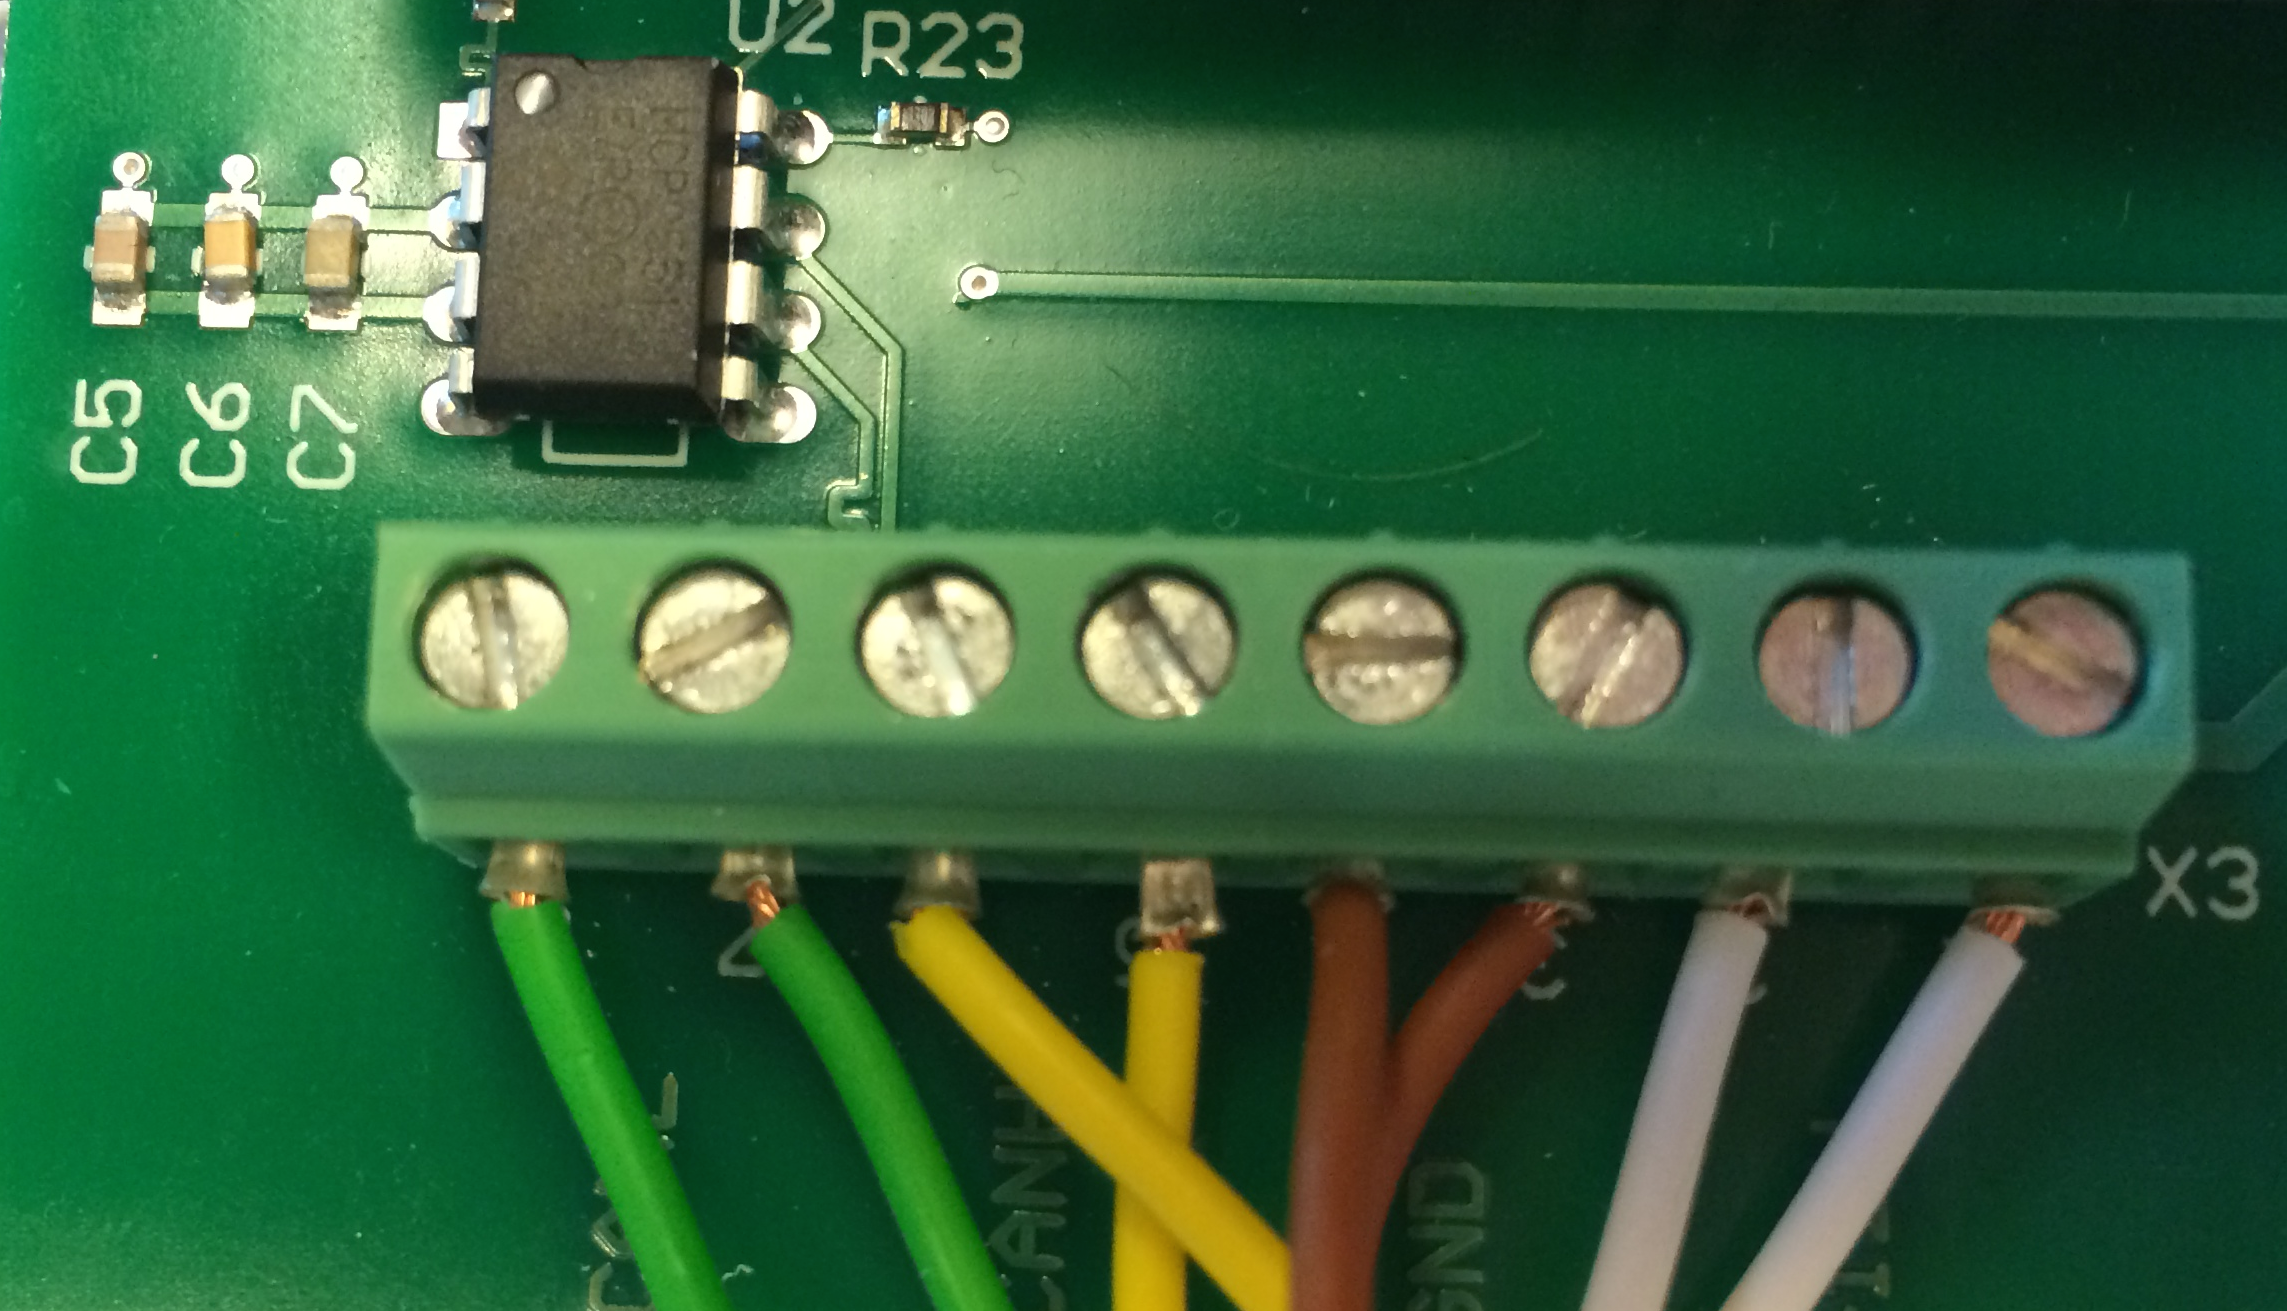
\includegraphics[width=0.8\textwidth]{images/AnschlussKabel.png}
	\caption{Anschluss der Leitungen an den Schraubklemmen.}
	\label{fig.kabel}
\end{figure}









\section{Ereignis}\label{sec.manualimpact}
Als Ereignis wird eine Signalform bezeichnet, die einem Einschlag eines Steins auf dem Sensor entspricht. Um Ereignisse zu erkennen, wird ein \gls{threshold} für den Signalpegel definiert. Wird dieser Wert überschritten, beginnt ein Ereignis. Sobald der Signalpegel für eine gewisse Zeit unterhalb des \gls{threshold}s geblieben ist, ist das Ereignis beendet. Das Verfahren der Ereigniserkennung wird im Abschnitt \ref{subsec.sw_ereignis} ab Seite \pageref{subsec.sw_ereignis} im Detail erklärt.

Ein Beispiel eines Ereignisses ist in Abbildung \ref{fig.impactraw} gegeben. Es handelt sich um den Einschlag eines Golfballs auf einer Aluminiumplatte, unter der der Beschleunigungssensor montiert ist. Die schwarz gestrichelten Geraden zeigen den \gls{threshold}, die roten Geraden zeigen den erkannten Anfang und Ende des \gls{ereignis}ses. Das Ende des \gls{ereignis}ses wird von der \gls{ereignisdet} auf jenen Messpunkt gelegt, an dem der Signalpegel den \gls{threshold} vor dem \gls{timeout} das letzte Mal unterschritten hat. Die Messwerte vor der dem \gls{timeout} werden je nach Detail-Level abgeschnitten. Die folgende Beschreibung der Detail-Level bezieht sich auf dieses Beispiel-Ereignis.

\begin{figure}
	\centering
		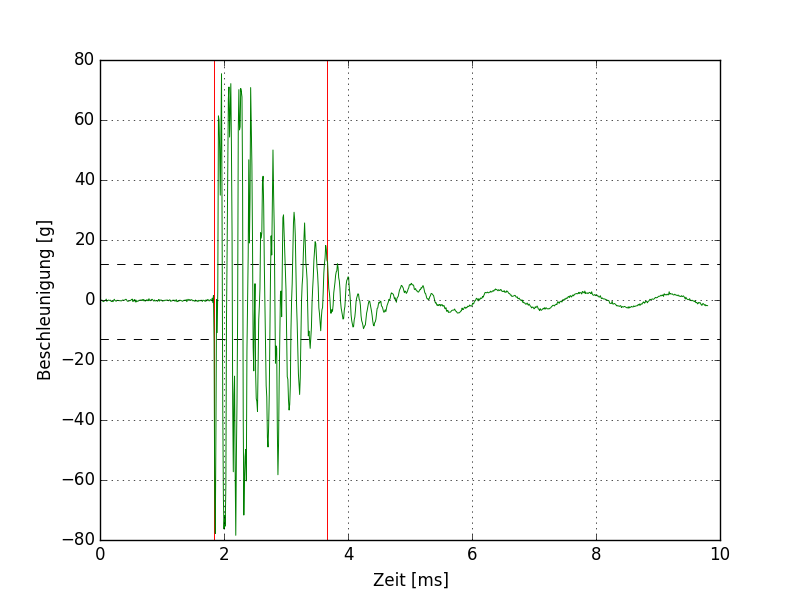
\includegraphics[width=0.8\textwidth]{images/raw.png}
	\caption{Beispiel von Rohdaten.}
	\label{fig.impactraw}
\end{figure}

\subsection{Detail-Level}\label{ssec.detaillevel}
Die Messstation kann Daten mit unterschiedlichen Detailgraden speichern. Jede \gls{sensoreinh} kann individuell auf einen Detail-Level konfiguriert werden.

\begin{itemize}
\item raw
\item detailed
\item peaks only
\item sparse
\item off
\end{itemize}


\subsubsection{Rohdaten (raw)}
Im Modus 'raw' werden Rohdaten ohne Ereigniserkennung übertragen und gespeichert. Es resultiert eine lückenlose Erfassung aller Messpunkte. Abbildung \ref{fig.detailraw} zeigt in Grün, welche Daten des Beispielereignisses im Modus 'raw' übertragen werden.


\begin{figure}
	\centering
		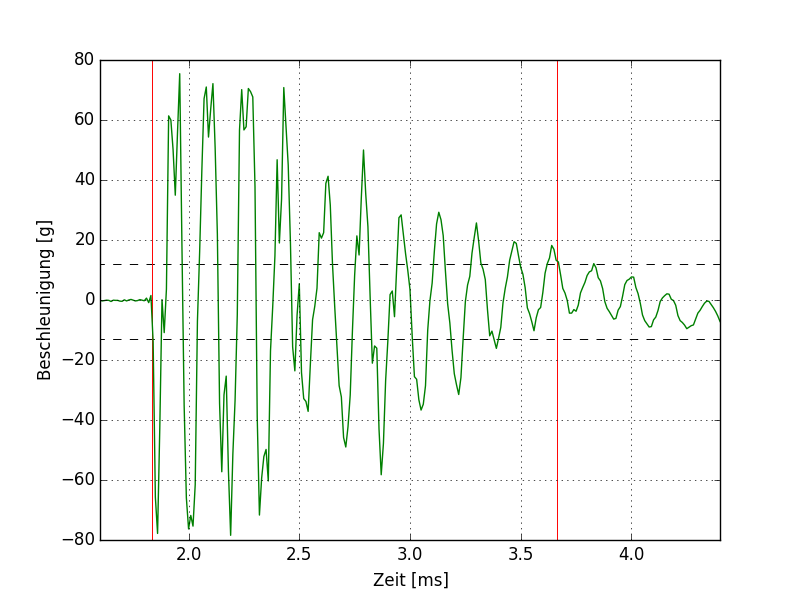
\includegraphics[width=0.8\textwidth]{images/rawshort.png}
	\caption{Detail-Level 'raw'.}
	\label{fig.detailraw}
\end{figure}

\paragraph{Datenaufkommen} Das Datenaufkommen ist in diesem Modus am grössten. Für jedes \gls{sample} wird ein 8-bit Wert abgespeichert. Bei einer \gls{fs} von 10000~Hz fallen also 10000~Byte Daten pro Sensor und Sekunde an.

\paragraph{Beispieldaten} \todo{beispieldaten einfügen}

\subsubsection{Detaillierte Ereignisdaten (detailed)}
Die \gls{ereignisdet} sucht den Beginn und das Ende des Ereignisses. Es werden sämtliche \glspl{sample} des Ereignisses übertragen. Im Konfigurationsmenü wird dieser Modus als 'detailed' bezeichnet. In Abbildung \ref{fig.detaildetailed} entspricht die grüne Kurve den gespeicherten Daten.

\begin{figure}
	\centering
		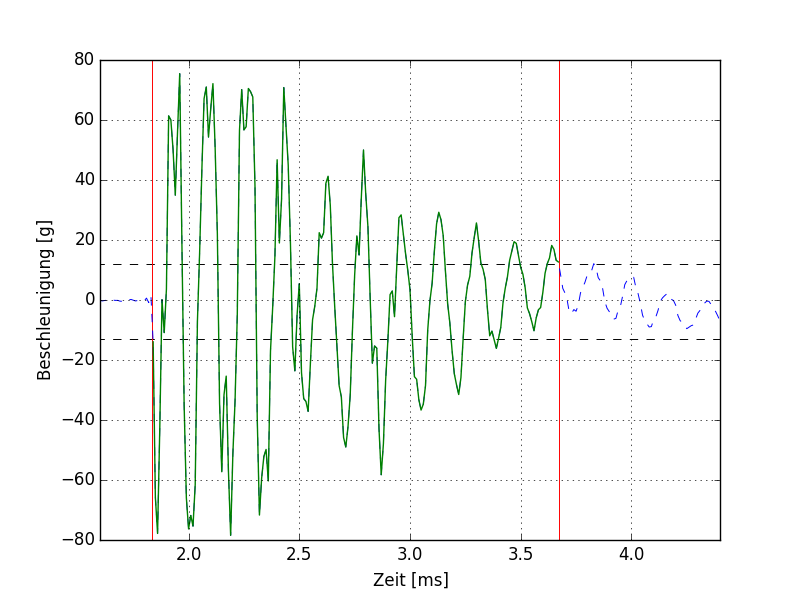
\includegraphics[width=0.8\textwidth]{images/detailed.png}
	\caption{Detail-Level 'detailed'.}
	\label{fig.detaildetailed}
\end{figure}

\paragraph{Datenaufkommen} Pro \gls{sample} wird ein Byte abgespeichert, der Startzeitpunkt und die Dauer belegen zusammen sechs Byte pro Ereignis. Die Datenmenge variiert mit der Dauer der Ereignisse. Es wird geschätzt, dass bei hohem Ereignisaufkommen während etwa 10~\% der Messzeit ein Ereignis vorliegt. Somit wird die Datenrate ungefähr ein Zehntel der \gls{fs} in Byte/Sekunde sein.

\paragraph{Beispieldaten} \todo{beispieldaten einfügen}

\subsubsection{Peaks (peaks only)}
Die Ereigniserkennung sucht im Modus 'peaks only' den Beginn und das Ende und somit die Dauer des Ereignisses. Ausserdem wird der maximale Ausschlag und alle Peakspitzen mit dem \gls{timestamp} und Höhe des Ausschlags gespeichert.
\begin{figure}
	\centering
		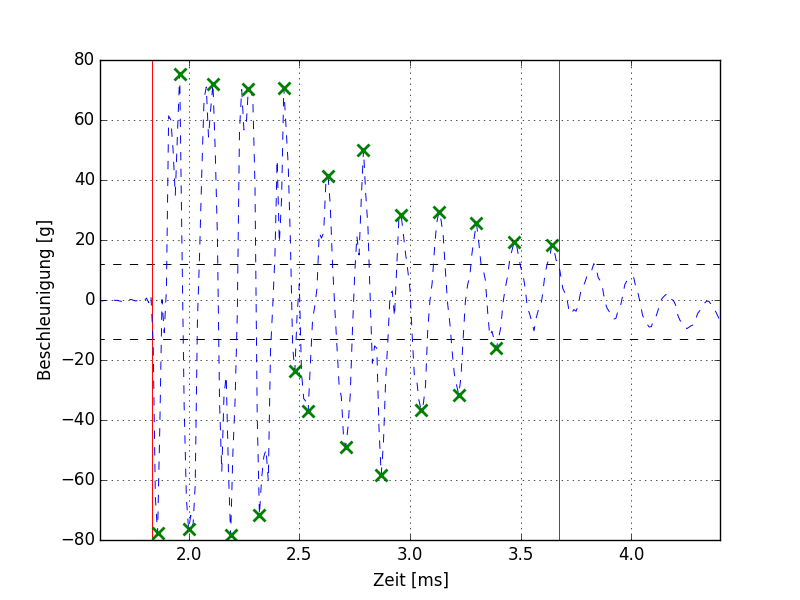
\includegraphics[width=0.8\textwidth]{images/peaks.png}
	\caption{Detail-Level 'peaks'.}
	\label{fig.detailpeaks}
\end{figure}

\paragraph{Datenaufkommen} Für die Eckdaten (Beginn, Dauer, Anzahl Peaks, maximaler Ausschlag) fallen 8 Byte Daten an. Jeder Peak benötigt zwei Byte: ein Byte für die Anzahl Samples seit dem letzten Peak und ein Byte für die Höhe des Ausschlags. In der Abbildung \ref{fig.detailsparse} zeigt die blau gestrichelte Linie den Verlauf der Messkurve, die roten Geraden markieren Beginn und Ende des \gls{ereignis}ses. Die grünen 'X' markieren die Peakspitzen, die übertragen werden.

\paragraph{Beispieldaten} \todo{beispieldaten einfügen}

\subsubsection{Minimale Daten (sparse)}
Im Modus 'sparse' werden nur Eckdaten des \gls{ereignis}ses gespeichert: Beginn und Dauer, Anzahl Peaks und maximaler Ausschlag. Dafür genügen acht Byte pro Ereignis. Die Eckdaten sind in Abbildung \ref{fig.detailsparse} dargestellt.

\begin{figure}
	\centering
		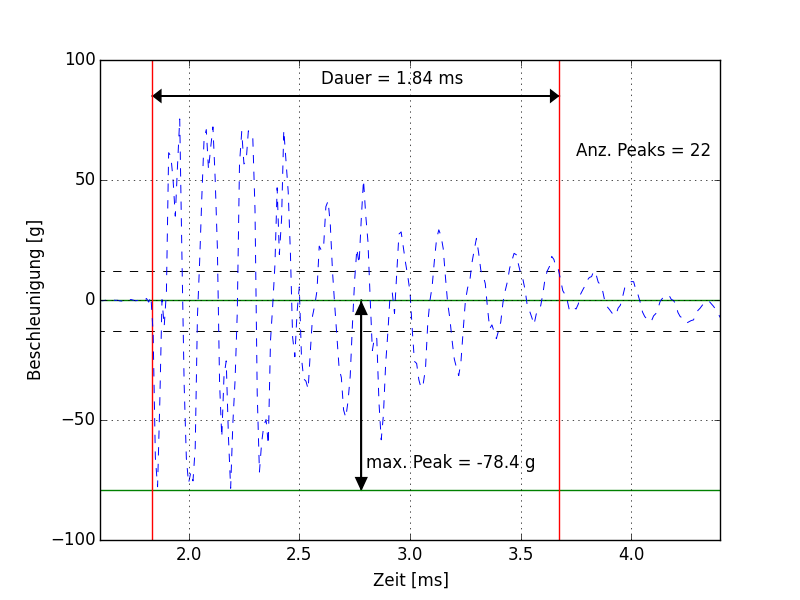
\includegraphics[width=0.8\textwidth]{images/sparse.png}
	\caption{Detail-Level 'sparse'.}
	\label{fig.detailsparse}
\end{figure}

\paragraph{Datenaufkommen} Der \gls{timestamp} für den Beginn des \gls{ereignis}ses benötigt vier Byte, die Dauer (Anzahl Samples) zwei Byte. Die Anzahl Peaks und der maximale Ausschlag belegen je ein Byte.

\paragraph{Beispieldaten} \todo{beispieldaten einfügen}

\subsubsection{Inaktiv (off)}
Die \gls{sensoreinh} kann in den Detail-Level 'off' gesetzt werden. In diesem Fall startet sie auch keine Messung, wenn der \gls{logger} alle \glspl{sensoreinh} startet.

In diesem Detail-Level fallen keine Daten an.


\section{Konfiguration}\label{sec.manualkonfig}


\subsection{Anschluss eines Computers}\label{ssec.manualserial}
Am \gls{usb}-Anschluss des \gls{logger}s kann ein \gls{compi} angeschlossen werden, um auf die serielle Schnittstelle des \gls{logger}s zuzugreifen. Um die serielle Schnittstelle zu verwenden, wird ein \gls{terminalemu} wie \emph{PuTTY} oder \emph{minicom} benötigt. um mit \emph{PuTTY} eine Verbindung aufzubauen, muss die Schnittstelle und die Übertragungsrate (Baud) angegeben werden. Die Übertragungsrate ist 9600 baud, die Schnittstelle kann variieren. 

\paragraph{Windows} Unter \emph{Windows} erfolgt die Verbindung auf eine der COMx-Schnittstellen. Die Nummer der COM-Schnittstelle kann im Geräte-Manager herausgesucht werden, die Bezeichnung lautet 'mbed Serial Port (COMx)', wobei 'x' eine Nummer ist. In PuTTY muss nur 'COMx' angegeben werden.

\paragraph{Linux} Unter \emph{Linux} findet man die Schnittstellenbezeichnung mit dem Befehl 'ls /dev/ttyACM*' heraus, in \emph{PuTTY} wird dann '/dev/ttyACMx' angegeben. 

\paragraph{Mac OS X} Unter \emph{Mac OS X} lautet der Befehl 'ls /dev/tty.usbmodem*', der in einem Terminal eingegeben werden muss. Als \gls{terminalemu} kann 'screen' verwendet werden. Auf Apple Mac Computern mit \gls{usb} 3.0 kann es zu Schwierigkeiten mit der Verbindung kommen. Den Herstellern des Prozessorboards ist dies bekannt, sie arbeiten an einer Lösung.

Die Einstellungen für die serielle Schnittstelle sind normalerweise bereits korrekt gesetzt. Es werden 8 Datenbits verwendet, 1 Stopbit und keine Parität (parity).

Weitere Hilfe für die Verwendung eines \gls{terminalemu}s findet man unter \url{http://developer.mbed.org/handbook/Terminals}.



\subsection{Menü}\label{ssec.menu}
Beim Herstellen der Verbindung über einen \gls{terminalemu} wird das Basis-Menü angezeigt. Durch Eingabe der Zahl wird der entsprechende Menü-Eintrag gewählt. Im Folgenden wird das gesamte Menü im Detail beschrieben.

Das Basis-Menü (siehe Listing \ref{list.basemenu}) listet alle Überwachungs- und Konfigurations-Möglichkeiten auf. 

\begin{lstlisting}[caption=, label=list.basemenu]
 1) list files
 2) format SD card
 3) mount SD card
 4) unmount SD card
 5) logger status
 6) start/stop logging
 7) sensor parameters
 8) sensor states
 9) reset timestamp
10) internal clock
11) config file
\end{lstlisting}

\paragraph{Dateien auflisten} Mit dem Befehl 'list files' wird eine Liste aller Dateien auf der SD-Karte angezeigt. Die Liste enthält die Dateigrösse sowie den Dateinamen, siehe Abschnitt \ref{sssec.listfiles}.

\paragraph{SD-Karte formatieren} Um die SD-Karte für den ersten Gebrauch vorzubereiten, sollte sie formatiert werden. Dies erfolgt von Vorteil auf einem \gls{compi}, kann aber auch im \gls{logger} mit dem Befehl 'format SD card' gemacht werden, siehe Abschnitt \ref{sssec.sdformat}.

\paragraph{SD-Karte anmelden} Nach dem Einsetzen einer SD-Karte erkennt der \gls{logger} dies normalerweise automatisch. Es kann jedoch vorkommen, dass der \gls{logger} auf die neue Karte aufmerksam gemacht werden muss. Dies erfolgt mit dem Befehl 'mount SD card', siehe Abschnitt \ref{sssec.sdmount}.

\paragraph{SD-Karte abmelden} Vor dem Entfernen der SD-Karte müssen alle Dateien geschlossen werden. Dies erfolgt mit dem Befehl 'unmount SD card', siehe Abschnitt \ref{sssec.sdunmount}.

\paragraph{Status des Datenloggers} Mit dem Befehl 'logger status' werden einige Betriebszustandsdaten des Datenloggers angezeigt, siehe Abschnitt \ref{sssec.loggerstate}.

\paragraph{Aufzeichnung starten/stoppen} Um die Aufzeichnung im ganzen System zu starten oder zu stoppen wird der Befehl 'start/stop logging' verwendet, siehe Abschnitt \ref{sssec.startstop}.

\paragraph{Sensor-Einstellungen} Mit dem Befehl 'sensor parameters' kann eine einzelne \gls{sensoreinh} oder alle \glspl{sensoreinh} zusammen konfiguriert werden. Siehe Abschnitt \ref{sssec.sensorparam}.

\paragraph{Status der Sensoreinheiten} Der Betriebszustand aller angeschlossenen \glspl{sensoreinh} kann mit dem Befehl 'sensor state' (siehe \ref{sssec.sensorstate}) aufgelistet werden.

\paragraph{Timestamp zurücksetzen} Um den Timestamp in allen \glspl{sensoreinh} auf Null zurückzustellen, wird der Befehl 'reset timestamp' verwendet. Siehe Abschnitt \ref{sssec.timestamp}.

\paragraph{Interne Uhr} Die interne Uhr wird mit den Befehl 'internal clock' eingestellt, Abschnitt \ref{sssec.intclock} beschreibt dies im Detail.

\paragraph{Konfigurations-Datei} Mit dem Befehl 'config file' wird die Konfiguration der Sensoren abgespeichert oderr aus einer Datei eingelesen, siehe Abschnitt \ref{sssec.configfile}.

\subsection{Befehle}\label{ssec.befehle}
\todo{dateiliste einfügen.}
\subsubsection{Dateiliste}\label{sssec.listfiles}
\begin{lstlisting}[caption=, label=list.]
HIER LISTE DER FILES EINFueGEN
 0) exit
\end{lstlisting}


\subsubsection{SD-Karte formatieren}\label{sssec.sdformat}
\begin{lstlisting}[caption=Untermenü SD-Karte formatieren, label=list.sdformat]
 1) confirm formatting of SD card.
    All data will be erased.
 0) cancel
\end{lstlisting}

Beim Formattieren werden alle Dateien auf der SD-Karte gelöscht, inklusive der Konfigurationsdatei mit allen Sensor-Einstellungen. Der Befehl 'format SD card' holt vor der Ausführung nochmals eine Bestätigung ein, ob sich der Benutzer wirklich sicher ist, dass er alle Dateien löschen will (Listing \ref{list.sdformat}). Während dem Formatieren wird die Meldung \ref{list.sdformatting} angezeigt.

\begin{lstlisting}[caption=Statusmeldung SD formatieren, label=list.sdformatting]
formatting SD Card
\end{lstlisting}

Sind beim Formatieren Fehler aufgetreten, erhält man die Fehlermeldung \ref{list.sdformatfail}. In diesem Fall sollte die Karte in einem \gls{compi} geprüft und formatiert werden.

\begin{lstlisting}[caption=Fehlermeldung SD formatieren, label=list.sdformatfail]
Formatting SD card FAILED. Please use a Computer to format the card.
\end{lstlisting}

Bei erfolgreicher Formatierung wird die Meldung \ref{list.sdformatsuccess} ausgegeben. 

\begin{lstlisting}[caption=Erfolgsmeldung SD formatieren, label=list.sdformatsuccess]
Formatting done
Returning to base menu.
\end{lstlisting}


\subsubsection{SD-Karte anmelden}\label{sssec.sdmount}
Damit Dateien auf die SD-Karte geschrieben werden können, muss sie vorher erkannt werden. Normalerweise geschieht dies, sobald die Karte eingesetzt wird. Wenn keine SD-Karte erkannt wird, wird dies im Basismenü angezeigt wie im Listing \ref{list.sdmountfail}. Durch den Aufruf des Befehls 'mount SD card' im Basismenü (Listing \ref{list.basemenu}) kann die eingesetzte SD-Karte angemeldet werden.

Nach erfolgreicher Anmeldung der SD-Karte wird das Basismenü angezeigt. 

Wenn keine SD-Karte erkannt werden kann, wird eine Fehlermeldung \ref{list.sdmountfail} ausgegeben.

\begin{lstlisting}[caption=Fehlermeldung SD-Karte anmelden, label=list.sdmountfail]
No SD card detected! Please insert card and try again!
\end{lstlisting}


\subsubsection{SD-Karte abmelden}\label{sssec.sdunmount}
Bevor die SD-Karte aus dem \gls{logger} entfernt wird, sollte sie abgemeldet werden. Der \gls{logger} schliesst bei diesem Vorgang alle geöffneten Dateien, um Datenverlust zu vermeiden. Da beim Abmelden der Karte die Aufzeichnung der Daten gestoppt wird, wird vorher eine Bestätigung verlangt (Listing \ref{list.sdunmount}).

\begin{lstlisting}[caption=Untermenü SD-Karte abmelden, label=list.sdunmount]
 1) unmount SD card
    This will stop logging and close all data files.
 0) cancel
\end{lstlisting}

Falls die Konfiguration der Sensoren verändert, aber noch nicht in die Konfigurationsdatei geschrieben wurde, wird eine Warnung angezeigt (Listing \ref{list.sdunmountwarn}). Die Konfiguration bleibt im Speicher des \gls{logger}s erhalten, so lange die Spannungsversorgung angeschlossen ist und kann auch auf der neuen SD-Karte gespeichert werden.

\begin{lstlisting}[caption=Warnung vor SD-Karte abmelden bei ungespeicherter Konfiguration, label=list.sdunmountwarn]
******************************************************************
* WARNING: sensor configuration data has not been saved to file! *
* If you want to save config to file, cancel now.                *
******************************************************************
\end{lstlisting}

\subsubsection{Logger-Status}\label{sssec.loggerstate}
Mit dem Befehl 'logger status' können einige Information über den \gls{logger} angezeigt werden.

\todo{logger status listing}
\begin{lstlisting}[caption=Untermenü Logger-Status, label=list.loggerstatus]
Time: Sat Dec 6 18:00:00 2014
Started?: 1
\end{lstlisting}


\subsubsection{Starten und stoppen der Aufzeichnung}\label{sssec.startstop}
Um die Datenspeicherung im \gls{logger} zu unterbrechen oder wieder zu starten wird der Befehl 'start/stop logger' verwendet. Beim Aufruf des Befehls wird ein Untermenü gemäss Listing \ref{list.startstop1} oder Listing \ref{list.startstop2} angezeigt.

\begin{lstlisting}[caption=Untermenü Stoppen der Aufzeichnung, label=list.startstop1]
 Logger is running.
 1) stop the logging.
 0) cancel
\end{lstlisting}

Da sich das Menü dem gegenwärtigen Zustand anpasst, sieht es bei gestoppter Aufzeichnung aus wie in Listing \ref{list.startstop2}.

\begin{lstlisting}[caption=Untermenü Starten der Aufzeichnung, label=list.startstop2]
 Logger is stopped.
 1) start the logging.
 0) cancel
\end{lstlisting}

Wenn die Aufzeichnung am Logger gestoppt wird, wird an alle \glspl{sensoreinh} der Befehl zum Aufzeichnungsstopp gesendet. Die Einstellungen zum Detailmodus bleiben in der \gls{sensoreinh} aber erhalten. Beim erneuten Starten der Aufzeichnung im Logger werden auch die \glspl{sensoreinh} wieder gestartet. Es besteht auch die Möglichkeit, einzelne \glspl{sensoreinh} zu stoppen (siehe Abschnitt \ref{sssec.sensorparam}). Eine gestoppte \gls{sensoreinh} bleibt auch beim Starten der Aufzeichnung am \gls{logger} gestoppt, da sie schon vor dem Stopp in diesem Zustand war.

\subsubsection{Sensor-Parameter}\label{sssec.sensorparam}
Die Parameter der Datenerfassung und Ereigniserkennung können für alle \glspl{sensoreinh} gemeinsam oder für jede \gls{sensoreinh} individuell eingestellt werden. Die Auswahl einer einzelnen oder aller \glspl{sensoreinh} erfolgt beim Einstieg in das Untermenü der Sensor-Parameter. Listing \ref{list.sensorsel} zeigt die Auswahl der Sensoren. Die Auswahlliste enthält gleich die aktuellen Werte der Parameter, damit man eine Übersicht hat.


\begin{lstlisting}[caption=Untermenü Sensor-Auswahl, label=list.sensorsel]
 Nr  SID  serial       fs threshold baseline timeout   detail
 1)    2  461bfdf6  10000       200     2047      30      raw
 2)    3  361509a5  10000       150     2000      20    peaks
 ...
 7)    8  1562a010  20000       400     2047      15 detailed
 
 #) Select a sensor from the list.
99) Select all sensors.
 0) cancel
\end{lstlisting}

Nach der Auswahl einer \gls{sensoreinh} gelangt man zur Auswahl des anzupassenden Parameters, Listing \ref{list.sensorparam}. Ist ein einzelner Sensor ausgewählt, werden hier noch einmal die aktuellen Werte der Parameter angezeigt.

\begin{lstlisting}[caption=Untermenü Sensor-Parameter, label=list.sensorparam]
 1) set sampling rate (current: 10000 Hz)
 2) set threshold value (current: 200)
 3) set baseline value (current: 2047)
 4) set timeout (current: 30)
 5) set detail level (current: peaks only)
 6) start or stop recording (current: started)
 0) exit
\end{lstlisting}

\paragraph{Abtastrate} Die Abtastrate legt fest, wie oft pro Sekunde ein Messwert vom Beschleunigungssensor eingelesen werden soll. Die \glspl{sensoreinh} können in einem Bereich zwischen \ensuremath{100 Hz} und \ensuremath{200000 Hz} messen. Die Abtastrate kann in Schritten von \ensuremath{100 Hz} eingestellt werden, Listing \ref{list.paramfs}.

Die Abtastrate hat einen wesentlichen Einfluss auf die zu übertragende und zu speichernde Datenmenge, die benötigte Rechenleistung. Davon wiederum hängt die Zeitspanne ab, wie lange die Messstation ohne Wartung betrieben werden kann. Es wird deshalb empfohlen, die Abtastrate nur so hoch einzustellen, wie es wirklich benötigt wird. Wie hoch dieser Wert ist, hängt stark von den geplanten Auswertungen ab.

\begin{lstlisting}[caption=Untermenü Abtastrate, label=list.paramfs]
 #) Enter sampling rate in Hz. (multiple of 100 Hz in range 100..200'000 Hz)
 0) cancel
\end{lstlisting}

Bei Eingabe einer ungültigen oder nicht unterstützten Abtastrate wird eine Fehlermeldung ähnlich Listing \ref{list.paramfserror} angezeigt.

\begin{lstlisting}[caption=Fehlermeldung bei ungültiger Abtastrate, label=list.paramfserror]
Sampling rate 220000 Hz not supported, too high.
\end{lstlisting}

Bei einer Änderung der Abtastrate wird automatisch der Timestamp zurückgesetzt, damit die Zuweisung der Messdaten zu einem Zeitpunkt weiterhin erfolgen kann.

\paragraph{Ereigniserkennung} Die \gls{ereignisdet} hat drei Parameter, die die Form der gesuchten \glspl{ereignis} bestimmen.  Abbildung \ref{fig.params} illustriert die Zusammenhänge zwischen \gls{threshold} und \gls{nullpegel} sowie die Funktionsweise des \gls{timeout}s.

\paragraph{Threshold} Der \gls{threshold} (Schwellenwert) ist ein Parameter der Ereigniserkennung. Er bestimmt, ab welcher Abweichung vom Nullwert ein Signal als Peak betrachtet werden soll. Bei der Wahl des \gls{threshold}s ist zu beachten, dass der \gls{threshold} auf beide Seiten des Nullwerts gilt. Daher darf die Summe des \gls{nullpegel}s und des \gls{threshold}s nicht den maximalen Wert (4096) des \gls{adwandler}s überschreiten. Ebenso muss der Wert des \gls{threshold}s kleiner sein als der \gls{nullpegel}, damit kein negativer Messwert anliegen müsste, um einen Peak zu erzeugen. Diese Einschränkungen werden bei der Eingabe noch einmal angezeigt, Listing \ref{list.paramthres}.

\begin{figure}
	\centering
		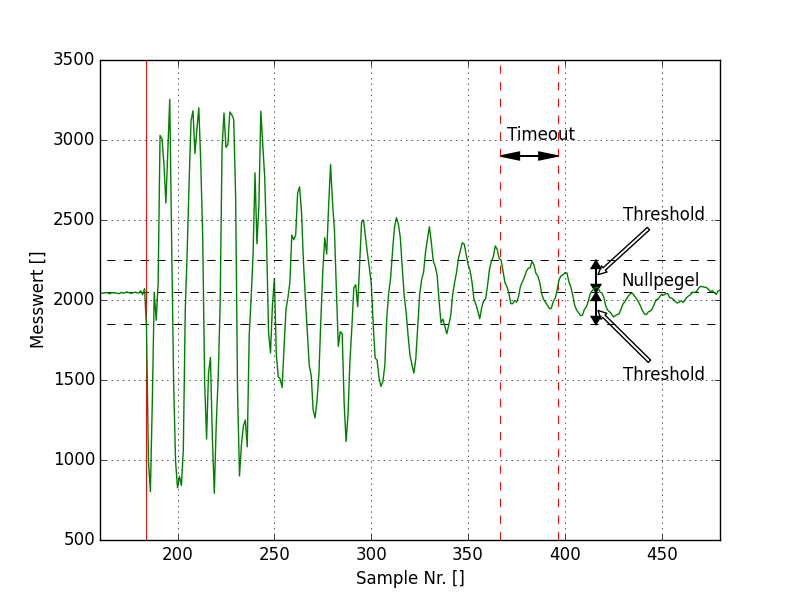
\includegraphics[width=0.8\textwidth]{images/impact_params.png}
	\caption{Zusammenhänge der Parameter der \gls{ereignisdet}.}
	\label{fig.params}
\end{figure}

\begin{lstlisting}[caption=Untermenü Threshold, label=list.paramthres]
 #) Enter threshold value.
    baseline + threshold must not exceed 4096
    and
    baseline - threshold must not be below 0
 0) cancel
\end{lstlisting}

Bei Verletzung der Kriterien für den \gls{threshold} wird eine entsprechende Fehlermeldung angezeigt, Listing \ref{list.paramthresfail}. Da die gleichen Kriterien auch bei der Einstellung des \gls{nullpegel}s gelten, empfiehlt es sich, zuerst einen kleinen Wert für den \gls{threshold} zu wählen. Dann kann der \gls{nullpegel} ohne grosse Einschränkung eingestellt werden. Danach setzt man den passenden \gls{threshold}.

\begin{lstlisting}[caption=Fehlermeldung ungültiger Threshold, label=list.paramthresfail]
 Invalid threshold value:
 threshold + baseline must not exceed 4096
 and
 threshold must be smaller than baseline value.
\end{lstlisting}

\paragraph{Nullpegel} Der \gls{nullpegel} wird mit einer ähnlichen Maske (Listing \ref{list.parambase}) wie der \gls{threshold} eingestellt, auch die Einschränkungen für den Wertebereich sind die Gleichen.

\begin{lstlisting}[caption=Untermenü Null-Level, label=list.parambase]
 #) Enter baseline value (default: 2047).
 0) cancel
\end{lstlisting}

Die Fehlermeldung bei ungültigen Werten für den \gls{nullpegel} ist in Listing \ref{list.parambaseerror} aufgeführt.

\begin{lstlisting}[caption=Fehlermeldung ungültiger Nullpegel, label=list.parambaseerror]
Invalid baseline value:
threshold + baseline must not exceed 4096.
and
threshold - baseline must not be below 0 value
\end{lstlisting}

\paragraph{Timeout} Der \gls{timeout} definiert, wie viele Samples der Signalwert unterhalb des \gls{threshold}s liegen kann, bevor das \gls{ereignis} als beendet betrachtet wird (Listing \ref{list.paramtimeout}). Die einzige Einschränkung an den \gls{timeout} ist, dass er die Länge des Ereignispuffers nicht überschreiten darf.
\todo{Länge des Ereignispuffers}

\begin{lstlisting}[caption=Untermenü Timeout, label=list.paramtimeout]
 #) Enter timeout in samples.
 0) cancel
\end{lstlisting}

Bei zu langem (Listing \ref{list.paramtimeoutlong}) oder sehr kurzem (Listing \ref{list.paramtimeoutshort}) \gls{timeout} wird eine Fehlermeldung resp. Warnung angezeigt.

\begin{lstlisting}[caption=Fehlermeldung zu langer Timeout, label=list.paramtimeoutlong]
Timeout too long, can not exceed 512.
\end{lstlisting}

\begin{lstlisting}[caption=Warnung kurzer Timeout, label=list.paramtimeoutshort]
Timeout 0 will end impact after each peak.
Timeout 0 in effect.
\end{lstlisting}

\paragraph{Detaillevel} Über die Wahl des Detaillevels wird bestimmt, wie viele und welche Daten von jedem \gls{ereignis} übertragen und gespeichert werden sollen (Listing \ref{list.detail}). Die Detaillevel sind geordnet nach anfallender Datenmenge, beginnend mit dem grössten Aufwand. Die Detaillevel sind in Abschnitt \ref{sec.manualimpact}, Seite \pageref{sec.manualimpact} beschrieben.

\begin{lstlisting}[caption=Untermenü Detail-Level, label=list.detail]
 1) raw (continuous data)
 2) detailed (start time, all samples of impact)
 3) peaks only (start time, nr of peaks, peaks
 4) sparse (only start time, duration, nr of peaks, max peak)
 5) off
 0) cancel
\end{lstlisting}

\paragraph{Start/Stop Sensor} Jede \gls{sensoreinh} kann einzeln gestartet oder gestoppt werden, vorausgesetzt der \gls{logger} ist gestartet. Im Untermenü ist ersichtlich, in welchem Zustand die ausgewählte \gls{sensoreinh} gerade ist (listing \ref{list.started_one}). Falls die Konfigurationsänderung alle \glspl{sensoreinh} betreffen soll, wird die Anzahl gestarteter und gestoppter Sensoren angezeigt (listing \ref{list.started_all}).

\begin{lstlisting}[caption=Untermenü Start/Stop einzeln, label=list.started_one]
Selected sensor is currently stopped.
 1) start
 2) stop
 0) cancel
\end{lstlisting}

\begin{lstlisting}[caption=Untermenü Start/Stop alle Sensoren, label=list.started_all]
Started sensors: 3
Stopped sensors: 0
 1) start
 2) stop
 0) cancel
\end{lstlisting}

Wenn ein Sensor gestartet wird, muss für die anfallenden Daten eine Datei erzeugt werden. Schlägt dies fehl, wird dies mit der Fehlermeldung \ref{list.sensorerror} angezeigt. Der Sensor wird dann nicht gestartet. Es wird empfohlen, in diesem Fall die SD-Karte zu überprüfen. Möglicherweise verfügt die SD-Karte nicht mehr über genügend Speicherplatz.

\begin{lstlisting}[caption=Fehlermeldung beim Starten eines Sensors, label=list.sensorerror]
Could not create or open file. Please check SD card for free space.
\end{lstlisting}

\subsubsection{Sensor-Status}\label{sssec.sensorstate}
Um die Einstellungen alles Sensoren auf einen Blick zu überprüfen, kann mit dem Befehl 'sensor states' die Liste aller Einstellungen aufgerufen werden, Listing \ref{list.sensorstatus}. In der Liste sind eine interne Nummer, die CAN-Bus-ID, die Seriennummer der \gls{sensoreinh} sowie alle Einstellungen aufgeführt.

\todo{TW: Liste von Sensor-Stati ins Listing einfügen}
\begin{lstlisting}[caption=Untermenü Sensor-Status, label=list.sensorstatus]
Listing sensor config:
 Nr  SID  serial       fs threshold baseline timeout     detail
 1)    2  461bfdf6  10000       200     2047      30        raw
 2)    3  361509a5  10000       150     2000      20 peaks only
 
 0) continue
\end{lstlisting}


\subsubsection{Timestamp zurücksetzen}\label{sssec.timestamp}
Der Timestamp kann manuell zurückgesetzt werden, dafür wird eine Bestätigung eingeholt: Listing \ref{list.timestamp}. Das Zurücksetzen des Timestamps betrifft immer alle \glspl{sensoreinh}.

\begin{lstlisting}[caption=Untermenü Timestamp zurücksetzen, label=list.timestamp]
 1) re-synchronize timestamp
 0) cancel
\end{lstlisting}


\subsubsection{Interne Uhr}\label{sssec.intclock}
Anhand der internen Uhr werden die Timestamps vom \gls{logger} in einen realen Zeitpunkt umgerechnet. Deshalb wird empfohlen, die interne Uhr auf die korrekte Uhrzeit einzustellen. Dies erfolgt über den Befehl 'internal clock', Listing \ref{list.intclock}. Hier kann das Datum (Untermenü \ref{list.setdate}) und die Tageszeit (Untermenü \ref{list.settime}) eingestellt werden.

\todo{Beispiel einer Uhrzeit einfügen}
\begin{lstlisting}[caption=Untermenü interne Uhr, label=list.intclock]
 1) adjust date
 2) adjust time
 0) exit

 current time: Sat Dec 6 18:00:00 2014
\end{lstlisting}

Das Einstellung des Datums erfolgt mit Inkrementen resp. Dekrementen von 365, 30, 10 Tagen oder 1 Tag.

\begin{lstlisting}[caption=Untermenü Datum einstellen, label=list.setdate]
adjust internal date
 1) adjust date +365 days
 2) adjust date -365 days
 3) adjust date + 30 days
 4) adjust date - 30 days
 5) adjust date + 10 days
 6) adjust date - 10 days
 7) adjust date +  1 day
 8) adjust date -  1 day
 0) exit

 current time: Sat Dec 6 18:00:00 2014
\end{lstlisting}

Die Uhrzeit wird mittels Inkrementen resp. Dekrementen von 1 Stunde, 10 oder 1 Minute oder 1 Sekunde eingestellt. Die aktuelle Uhrzeit wird jeweils unterhalb des Menüs angezeigt.

\begin{lstlisting}[caption=Untermenü Uhrzeit einstellen, label=list.settime]
adjust internal time
 1) adjust time +1 hour
 2) adjust time -1 hour
 3) adjust time +10 minute
 4) adjust time -10 minute
 5) adjust time +1 minute
 6) adjust time -1 minute
 7) adjust time +1 second
 8) adjust time -1 second
 0) exit

 current time: Sat Dec 6 18:00:00 2014
\end{lstlisting}

\subsubsection{Konfigurations-Datei}\label{sssec.configfile}

Über den Befehl 'config file' (Listing \ref{list.configfile}) kann die aktuelle Konfiguration der \glspl{sensoreinh} in die Konfigurationsdatei 'config.txt' abgespeichert werden, oder eine neue Konfiguration aus der Datei eingelesen und an die \glspl{sensoreinh} gesendet werden. Es ist nicht möglich, aus mehreren Konfigurationsdateien auszuwählen.
\todo{mehrere konfig-files und file löschen könnte man in den Ausblick nehmen, als zu verbessernde punkte}

\begin{lstlisting}[caption=Untermenü Konfigurationsdatei, label=list.config]
 1) read configuration from file and set up all sensors accordingly.
 2) store current configuration in file. Old config file will be overwritten.
 0) cancel
\end{lstlisting}

Falls die Konfigurationsdatei nicht gespeichert werden kann, wird die Fehlermeldung in Listing \ref{list.configerror} angezeigt. Um die Konfigurationsdatei trotzdem speichern zu können, kann die SD-Karte abgemeldet und ausgetauscht werden. Die Konfiguration bleibt erhalten, so lange die Spannungsversorgung besteht.

Um einem möglichen Konfigurationsdatenverlust vorzubeugen empfiehlt es sich, die Konfigurationsdatei zu speichern, sobald alle Einstellungen wie gewünscht gemacht wurden. Nach einem Unterbruch in der Spannungsversorgung wird nach automatisch die Konfiguration aus der 

\begin{lstlisting}[caption=Fehlermeldung beim Speichern der Konfigurationsdatei, label=list.configerror]
The config file could not be written. Please check the SD card in a computer.
The configuration data will remain stored in the logger unless you turn off power.
\end{lstlisting}

\subsection{Konfigurationsdatei}
In der Konfigurationsdatei werden die Einstellungen der \glspl{sensoreinh} gespeichert. Die Datei kann auch auf einem \gls{compi} erstellt werden und über eine SD-Karte auf den \gls{logger} übertragen werden. Ein Beispiel einer Konfigurationsdatei zeigt Listing \ref{list.configfile}. Die erste Zeile enthält die Anzahl Datensätze. Jeder Datensatz enthält die Konfiguration einer \gls{sensoreinh}. Auf der zweiten und den folgenden Zeilen folgen die Datensätze. 

Ein Datensatz enthält die CAN-Bus-ID, die Seriennummer der \gls{sensoreinh} als Hexadezimalzahl, die \gls{fs} (ohne die hintersten zwei Nullen), den \gls{threshold}, den \gls{nullpegel} und den \gls{timeout} sowie den Detail-Level und ob der Sensor Daten aufzeichnen soll (1) oder nicht (0).

Der \gls{logger} versucht nach dem Einschalten der Spannungsversorgung die Konfigurationsdatei von der SD-Karte zu lesen. Falls keine SD-Karte vorhanden ist, startet der \gls{logger} den Betrieb nicht, da keine Messdaten gespeichert werden können. Falls die SD-Karte vorhanden ist, aber keine Konfigurationsdatei 'config.txt' enthält, startet der Betrieb der Messstation im Standardmodus.

\paragraph{Standardmodus} Im Standardmodus arbeiten alle \glspl{sensoreinh} mit einer \gls{fs} von \ensuremath{10000 Hz}, \gls{threshold} 200, \gls{nullpegel} 2047, \gls{timeout} 30. Der Detail-Level wird auf 'peaks only' gesetzt, siehe Abschnitt \ref{sec.manualimpact}, Seite \pageref{sec.manualimpact}. Alle \glspl{sensoreinh} werden gestartet.

\begin{lstlisting}[caption=Beispiel einer Konfigurationsdatei, label=list.configfile]
{3,
{2, 461bfdf6, 100, 200, 2047, 30, 3, 1},
{3, 15047b39, 100, 150, 2040, 30, 2, 1},
{4, b78d6dca, 100, 100, 2049, 30, 4, 1},
}
\end{lstlisting}

Falls Änderungen an der Konfiguration gemacht, aber nicht in die Konfigurationsdatei geschrieben wurden, erscheint im Basismenü die Information gemäss Listing \ref{list.configinfo}.

\begin{lstlisting}[caption=Information bei ungespeicherter Konfiguration, label=list.configinfo]
Config has been modified but not saved to SD card.
\end{lstlisting}

